\subsection{Gap 5: Single-Objective Optimization Assumptions}
\label{sec:multiobjective}

\subsubsection{Findings}

All frameworks optimize single objectives or use fixed weighted sums. No framework supports Pareto optimization, constraint satisfaction, or uncertainty-aware candidate selection. Task class 15 (safety/toxicology modeling with multi-objective trade-offs) receives only partial coverage: five of six frameworks provide adjacent capabilities (toxicophore flagging, ADMET prediction) but none supports multi-objective trade-off reasoning, Pareto optimization, or dose-response modeling.

\subsubsection{Analysis}

Resource constraints amplify the cost of poor decisions. When every experiment is precious, navigating multi-objective trade-offs becomes critical. Consider three peptide candidates from a development campaign. One shows tenfold higher proliferation bioactivity but triggers hepatotoxicity at effective doses. Another has half the bioactivity but higher tolerated dosing, yielding comparable efficacy with better safety. A third has intermediate bioactivity and safety but superior stability enabling less frequent dosing. "Optimal" depends on patient population, dosing regimen, and regulatory risk tolerance. No single metric captures this.

Drug discovery is multi-objective optimization: candidates must satisfy bioactivity, selectivity, safety, stability, manufacturability, and cost. Objectives conflict: potency improvements reduce selectivity, stability enhancements increase immunogenicity, high-purity synthesis is expensive. Navigating requires understanding Pareto frontiers (candidates where improving one objective degrades another) and decisions based on risk tolerance, development stage, and context.

Current agents optimize single objectives. ChemCrow optimizes binding affinity or synthetic accessibility \citep{bran2024chemcrow}. Coscientist targets synthesis yield \citep{boiko2023coscientist}. Multiple objectives collapse to weighted sums: "Maximize 0.6×bioactivity + 0.4×drug-likeness" \citep{bickerton2012qed}. This discards information: which candidates are Pareto-optimal, how sensitive are rankings to weights, what trade-offs exist. Agents present single "optimal" solutions, obscuring decision spaces.

\subsubsection{The Single-Metric Trap}

Single-metric optimization mirrors ML training objectives: minimize loss, maximize accuracy. This works for unidimensional goals, but drug discovery is multidimensional and context-dependent. Optimality depends on indication, development stage, competitive landscape, and risk tolerance.

Peptide stability illustrates the trap. A peptide that degrades rapidly in serum has no value. Stability modifications (D-amino acids, non-natural residues, cyclization) improve half-life but can reduce affinity, increase aggregation, or complicate synthesis. The balance depends on route of administration, therapeutic window, and development timeline.

Agents cannot represent these trade-offs. They predict A $>$ B but cannot articulate: "A is twice as potent but has a threefold narrower safety margin; choose A if dosing can be tightly controlled, choose B for robustness." They do not visualize Pareto frontiers or sensitivity to weight changes.

\subsubsection{Pareto Frontiers and Constraint Satisfaction}

\begin{figure}[htbp]
\centering
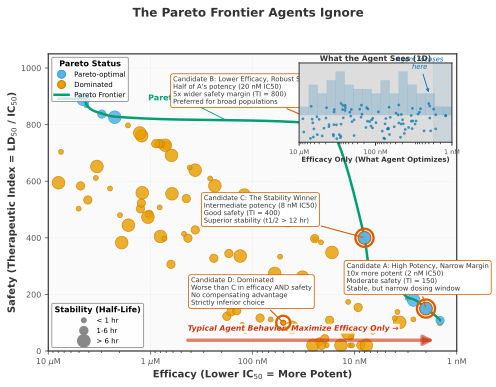
\includegraphics[width=\textwidth]{figures/fig6-pareto-frontier.jpeg}
\caption{The Pareto Frontier Agents Ignore. Two-dimensional scatter plot of candidate compounds across efficacy (IC50) and safety (LD50 ratio), with stability (half-life) encoded by point size. The Pareto frontier curve identifies candidates where improving one objective requires degrading another. Annotations show real decision trade-offs: lower efficacy but much safer, highly effective but stability concerns. Current single-objective optimization (red arrow pointing to maximum efficacy) misses this complexity.}
\label{fig:pareto}
\end{figure}

Pareto optimization is the appropriate framework. A candidate is Pareto-optimal if no other improves one objective without degrading another. The Pareto frontier is a curve (two objectives) or surface (three+). Practitioners navigate this frontier based on context.

Frontier visualization reveals trade-off structure. Steep regions require large sacrifices for modest gains; flat regions allow improvements with minimal cost. Clusters suggest distinct strategies (high-potency narrow-margin versus moderate-potency wide-margin). Gaps reveal unexplored regions.

Constructing the frontier requires multi-objective optimization. NSGA-II maintains candidate populations and selects non-dominated solutions. Multi-objective Bayesian optimization models objectives, selects candidates via acquisition functions balancing exploration and Pareto improvement, and updates with experimental results. These require tight integration between generative models, predictive models, and optimizers, which agents do not support.

Standalone multi-objective tools are advancing. PMMG \citep{pmmg2025} uses Pareto-guided Monte Carlo Tree Search to generate molecules satisfying seven simultaneous objectives with a 51.65\% success rate, outperforming baselines by 2.5 times. CheapVS \citep{cheapvs2025} enables human-guided preferential multi-objective Bayesian optimization, allowing chemists to express trade-off preferences via pairwise comparisons. These are effective optimization algorithms, but they are not integrated into agentic workflows providing uncertainty quantification, sensitivity analysis, stage-adaptive recommendations, and interactive decision support across iterative design cycles.

Constraints add complexity: synthesizability, solubility, permeability, absence of toxicophores. Constrained optimization identifies the Pareto frontier within feasible regions, which may be disjoint or conflicting. In peptide design, synthesis feasibility is often binding. Sequences with non-natural residues may be predicted optimal but are unavailable or prohibitively expensive. Regioselective cyclization can be unfeasible. Practitioners must balance optimization with synthetic pragmatism.

\subsubsection{Incorporating Uncertainty and Risk}

Predictions include uncertainty. IC50 equals 10 nM might have a 95% interval of 5-20 nM or 1-100 nM. Ignoring uncertainty leads to poor decisions: selecting high predicted activity with wide uncertainty and failing in validation. Incorporating uncertainty into multi-objective decisions is a standard requirement in Bayesian decision theory but is absent from current agents.

Bayesian optimization handles uncertainty via Gaussian processes providing means and variances. Acquisition functions (expected improvement, upper confidence bound) balance exploitation and exploration. Over rounds, uncertainty shrinks in explored regions and stays high elsewhere. Visualizing uncertainty to guide exploration versus exploitation is a key capability gap.

Risk profiles vary by stage. Early discovery tolerates high-risk, high-reward candidates. Late-stage demands well-characterized properties and high confidence. Effective frameworks would adapt recommendations accordingly.

In peptide pipelines, early rounds prioritized diversity, middle rounds balanced exploration and exploitation, final rounds focused on de-risking. This requires dynamic acquisition functions and explicit risk management absent from agents.

Sensitivity analysis is missing. How robust are rankings to model error? If bioactivity predictions have 20% error or toxicity is biased optimistic, which candidates remain Pareto-optimal? Sensitivity analysis quantifies robustness and guides resource allocation.

\subsubsection{Derived Requirements}

Closing this gap requires multi-objective Bayesian optimization with constraint handling, Pareto frontier visualization with interactive filtering, uncertainty quantification providing epistemic uncertainty in bioactivity prediction and dose-response confidence bands, and risk-aware candidate selection that adapts recommendations to development stage. The gap analysis identifies Pareto frontier representation, uncertainty quantification, risk-aware decision support, and structured decision spaces as design requirements, replacing the current pattern of outputting single optima.
